

 La administración educativa moderna requiere de herramientas tecnológicas capaces de transformar datos operativos en información estratégica. El presente documento detalla el diseño y desarrollo de la Plataforma de Análisis Estadístico para la Dirección Académica Escolar, un sistema integral creado para optimizar la toma de decisiones institucionales mediante la automatización y el procesamiento centralizado de datos. El objetivo principal de esta plataforma es agilizar la gestión y el análisis de indicadores académicos críticos. 
 El sistema abarca módulos fundamentales para el entorno escolar, tales como el seguimiento de la matrícula, eficiencia, rendimiento, procesos de titulación, asignación de becas, caracterización estudiantil y evaluaciones docentes. Para proporcionar una perspectiva analítica precisa y evaluar la evolución de la institución, la plataforma consolida y analiza información histórica a un plazo de 3 años hacia el pasado, permitiendo así identificar tendencias, ciclos generacionales y áreas de oportunidad con base en datos reales.  
 A través de una arquitectura robusta —que contempla el procesamiento de datos en segundo plano, validación de cargas masivas de archivos y la generación dinámica de reportes—, el proyecto busca eliminar los cuellos de botella asociados al manejo manual de la información. Los siguientes apartados de este documento profundizan en las especificaciones, requerimientos de software, arquitectura del sistema y las decisiones tecnológicas implementadas para consolidar esta solución en beneficio de la administración escolar.




\section{Antecedentes}

La Dirección Académica de la Universidad Politécnica de Texcoco ha enfrentado históricamente el reto de gestionar un volumen creciente de información escolar sin contar con una herramienta informática centralizada y especializada para el análisis estadístico de sus indicadores clave. 
Tradicionalmente, el almacenamiento y la administración de los datos institucionales se han delegado en hojas de cálculo electrónicas, específicamente archivos de Microsoft Excel. Si bien este método ha sido una solución accesible para el registro inicial de datos, 
la escala operativa de la universidad ha superado las capacidades de esta herramienta, debido a que la información correspondiente a la matrícula, la asignación de becas, el rendimiento, la eficiencia terminal, los ciclos generacionales y los procesos de titulación se encuentra dispersa en múltiples archivos individuales, cada uno estructurado con complejas estructuras de varias hojas de trabajo. 
Esta fragmentación de la información provoca que cuando surge la necesidad de consultar datos específicos o consolidados, el personal académico deba navegar de forma manual a través de decenas de pestañas y archivos independientes, volviendo el proceso de búsqueda y manejo de información sumamente tedioso, propenso a errores humanos y tardado, lo que disminuye drásticamente la capacidad de respuesta institucional. Asimismo, la evaluación del desempeño escolar requiere analizar la evolución académica con una perspectiva de al menos tres años hacia el pasado. 
Realizar este análisis histórico cruzando múltiples hojas de cálculo incrementa exponencialmente el riesgo de duplicidad, pérdida de consistencia en los datos y errores en la aplicación de fórmulas estadísticas, además de impedir la generación dinámica e inmediata de reportes ejecutivos o tableros visuales para los directivos.
\newpage

1. \textbf{Romero Alepuz, J. (2026). Dashboard web para la gestión y visualización dinámica de datos heterogéneos. Universitat Oberta de Catalunya (UOC).}

En este proyecto de titulación se presenta el diseño y desarrollo de un tablero de control (dashboard) web dinámico, el cual fue creado con la finalidad de recopilar y mostrar visualmente información que proviene de diferentes fuentes externas independientes. 
El objetivo principal de este sistema fue ofrecer una herramienta interactiva de autoservicio que funcione como una alternativa viable frente a las plataformas comerciales complejas y a las soluciones estáticas basadas en plantillas tradicionales, permitiendo que los usuarios configuren sus propios paneles de 
indicadores sin la necesidad de contar con conocimientos avanzados de programación. El resultado final de la investigación demuestra la viabilidad de centralizar datos que originalmente se encuentran desordenados o dispersos dentro de un único punto de control seguro, modular y escalable que  
agiliza el monitoreo de la información.


2. \textbf{Andrango, K. (2024). Dashboard estadístico sobre la publicación de datos abiertos por parte de las Instituciones de la Función Ejecutiva en el portal de datos abiertos del Ecuador.}

Este trabajo de titulación se centra en la propuesta y el desarrollo de un panel estadístico diseñado para resolver la falta de control y la poca claridad en la gestión de datos de distintas instituciones públicas. 
La problemática que motivó esta investigación radicaba en que la información se presentaba de forma muy general, lo que impedía supervisar de manera efectiva el cumplimiento y avance real de cada dependencia. 
Para solucionar esto, el autor estructuró un sistema basado en dos reportes clave: el primero reemplaza las cifras generales por una visión específica y detallada que proporciona una representación numérica exacta de los registros; mientras que el segundo reporte funciona 
como un mecanismo de monitoreo integral para rastrear el desempeño de cada institución. El proyecto demuestra cómo un panel de indicadores centralizado promueve la transparencia y facilita la comprensión de grandes volúmenes de información, transformando datos dispersos en informes visuales resumidos
 que apoyan directamente la rendición de cuentas.

\begin{figure}[H]
    \centering
    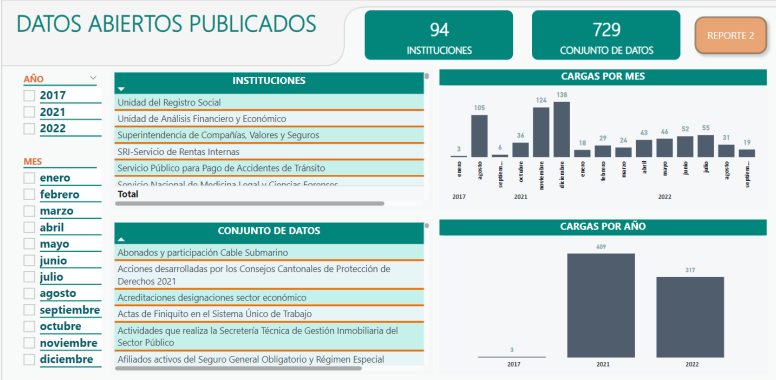
\includegraphics[width=0.8\linewidth]{imagenes/anexo2.png}
    \caption{Dashboard estadístico sobre la publicación de datos abiertos por parte de las Instituciones de la Función Ejecutiva en el portal de datos abiertos del Ecuador}
    \label{fig:dashboard_anexo2}
\end{figure}

3. \textbf{Rangel Narváez, A. (2016). Programación de un Web Dashboard para la presentación de estadísticas en una empresa. Facultad de Ciencias, Universidad Nacional Autónoma de México (UNAM).}

En este proyecto profesional se aborda la necesidad de optimizar la administración de los datos históricos de operación dentro de una organización, partiendo del principio de que esta información es el recurso más valioso para medir el comportamiento de un entorno y guiar su rumbo. 
El autor explica que el almacenamiento tradicional en registros individuales genera serios inconvenientes para el personal, ya que extraer la información requiere conocimientos técnicos avanzados y organizar millones de datos de forma manual vuelve muy lenta la entrega de reportes. 
Para resolver esta situación, se programó una plataforma web interactiva con gráficos, tablas y alertas que consolidan las métricas en un solo lugar con el fin de ofrecer una visión clara para el análisis de operaciones y la toma de decisiones rápidas. El desarrollo demuestra cómo automatizar las rutinas de cálculo para que la información esté actualizada constantemente y disponible para ser consultada a través de internet.
\newpage
4. \textbf{Martínez Luna, I. (2024). Elaboración de un dashboard, aplicado a la minería de datos para el apoyo a la toma de decisiones en el departamento de ventas. Facultad de Estudios Superiores Cuautitlán, UNAM.}

En esta tesis de licenciatura se analiza la problemática de las organizaciones que aún gestionan su información mediante procesos tradicionales y manuales, lo que genera retrasos en la elaboración de reportes, inconsistencia en los datos y poca confiabilidad al momento de evaluar los resultados. 
Para optimizar este flujo de trabajo, el autor implementó una metodología sistemática orientada a descubrir conocimiento dentro de las bases de datos, permitiendo transformar la información cruda en reportes consistentes dirigidos a los altos mandos. 
El proyecto consistió en diseñar un almacén de datos centralizado para reunir la información que se encontraba dispersa en múltiples hojas de cálculo, aplicando un proceso de limpieza para corregir las capturas erróneas antes de realizar la carga final. 
El resultado permite automatizar los informes y aplicar modelos estadísticos avanzados para encontrar patrones, tendencias y proyecciones relevantes representadas en forma gráfica y resumida.

\begin{figure}[H]
    \centering
    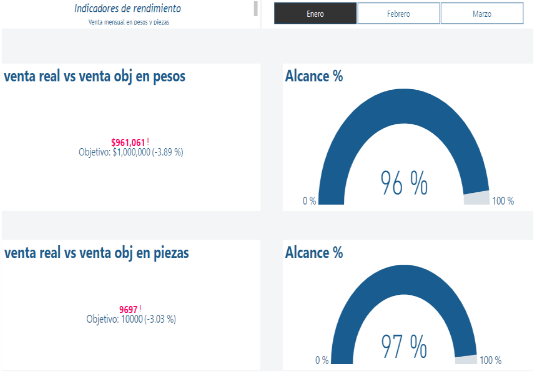
\includegraphics[width=0.8\linewidth]{imagenes/anexo3.png}
    \caption{Dashboard para departamento de ventas}
    \label{fig:dashboard_anexo3}
\end{figure}

\section{Planteamiento del problema}

En la Universidad Politécnica de Texcoco, el área de Dirección Académica tiene la tarea de controlar y revisar datos muy importantes, como la cantidad de alumnos que entran y salen, el rendimiento académico de los estudiantes, la eficiencia terminal, la titulación, las becas y las evaluaciones. 
Toda esta información sirve para que las autoridades de la escuela puedan planear mejoras y saber qué pasos dar en el futuro. 
\begin{figure}[H]
    \centering
    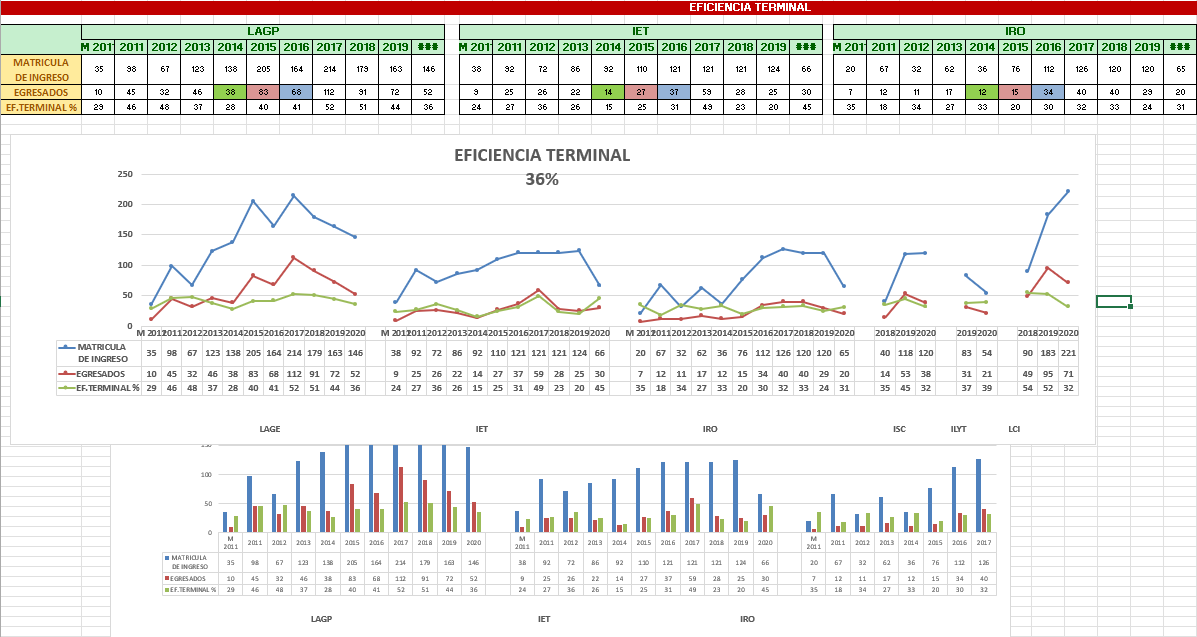
\includegraphics[width=0.8\linewidth]{imagenes/anexo1.png}
    \caption{Análisis de la situación actual}
    \label{fig:situacion_actual_anexo1}
\end{figure}
El gran detalle es que hoy en día todo este registro se hace a mano guardando los datos en archivos de Excel individuales. 
Aunque este sistema ha servido por un tiempo, la realidad es que trabajar así provoca muchos dolores de cabeza: es facilísimo cometer errores al escribir los datos, buscar información se vuelve una tarea muy pesada y las tablas no permiten ver los cambios de forma rápida o directa. 
Esto hace que sea muy difícil notar a tiempo cosas urgentes, como qué alumnos están a punto de dejar la escuela o en qué cuatrimestres específicos los estudiantes están bajando sus calificaciones y necesitan apoyo extra. No contar con un programa moderno e inteligente en la oficina de Dirección Académica frena la posibilidad de vigilar cómo va la universidad día con día. 
En la actualidad, para poder armar un informe o hacer una comparación de datos, el personal tiene que revisar manualmente carpetas llenas de hojas de cálculo, lo que quita muchísimo tiempo y retrasa la entrega de respuestas a los directivos. 
Además, tener la información regada por tantas partes complica juntarla toda en un solo lugar y bloquea la oportunidad de hacer estudios más completos a través de los años, como ver si los cambios que ha hecho la escuela realmente han servido a lo largo del tiempo. Todo esto afecta directamente la administración de la universidad, ya que las decisiones tardan en tomarse y se vuelve muy difícil proponer mejoras basadas en datos reales y ordenados.


\section{Justificación}

La gestión eficiente de la información académica es un factor crítico para el desarrollo y la mejora continua de cualquier institución de educación superior. Cuatrimestre a cuatrimestre, la Universidad Politécnica de Texcoco genera una cantidad masiva de datos vitales, tales como registros de matrícula, índices de reprobación y deserción, tasas de eficiencia terminal y resultados de las evaluaciones docentes. Sin embargo, el almacenamiento y análisis de esta información a través de hojas de cálculo aisladas y archivos de texto plano (CSV) presenta limitaciones significativas. Este manejo manual no solo hace que la consolidación de los datos sea un proceso lento y susceptible a errores humanos, sino que dificulta la visualización rápida de tendencias históricas, retrasando la capacidad de respuesta administrativa.

El desarrollo de este sistema web de indicadores institucionales se justifica por la necesidad imperante de modernizar, centralizar y automatizar el procesamiento de dichos datos. Al implementar una plataforma tecnológica que ingiera directamente los archivos estructurados y los transforme en tableros interactivos (dashboards), se elimina la redundancia operativa y se garantiza la integridad de la información. Esto permitirá a los coordinadores y directivos realizar cruces de información complejos en cuestión de segundos, como comparar el desempeño docente con los índices de aprovechamiento, o consultar el histórico de titulación de las últimas generaciones sin necesidad de buscar en múltiples archivos físicos o digitales.

Además del ahorro sustancial en tiempos de procesamiento administrativo, el mayor impacto de este proyecto radica en su aporte a la toma de decisiones. Dotar a la Universidad Politécnica de Texcoco de una herramienta de inteligencia de datos con control de acceso seguro asegurará que las autoridades cuenten con métricas precisas, actualizadas y fáciles de interpretar. En consecuencia, la institución tendrá una base empírica sólida para fundamentar sus estrategias de retención estudiantil, evaluar la calidad de sus programas educativos, facilitar auditorías y, en última instancia, elevar su nivel de excelencia académica.


 \section{Objetivo General}

Desarrollar un sistema web para el análisis y visualización de indicadores institucionales de la Universidad Politécnica de Texcoco, que permita la ingestión automática de datos académicos y administrativos, su procesamiento mediante rutinas estadísticas, y la representación de resultados con gráficos dinámicos, con el fin de facilitar la toma de decisiones basada en evidencia y mejorar la gestión estratégica de la institución.

\subsection{Objetivos especificos:}

\begin{itemize}
    \item Analizar y estructurar los conjuntos de datos históricos de la institución (archivos CSV de matrícula, aprovechamiento, titulación y evaluación docente) para diseñar el modelo de base de datos relacional que soportará el sistema.
\end{itemize}

 \begin{itemize}
     \item Desarrollar rutinas de procesamiento estadístico y métricas (eficiencia terminal, índice de reprobación, análisis de evaluación docente) capaces de ejecutarse automáticamente tras la carga de nuevos datos, generando indicadores actualizados en tiempo real.
 \end{itemize}

 \begin{itemize}
     \item Implementar una interfaz web responsiva con visualización de datos mediante gráficos interactivos (tableros tipo dashboard) que faciliten la interpretación de indicadores clave y la comparación histórica de métricas institucionales.
 \end{itemize}

 \begin{itemize}
     \item Establecer un sistema de autenticación y perfiles de usuario seguro para restringir el acceso a información sensible y permitir que cada usuario interactúe únicamente con las funcionalidades pertinentes.
 \end{itemize}

 \begin{itemize}
     \item Ejecutar pruebas integrales de rendimiento, validación de datos y usabilidad para verificar que la generación de las gráficas interactivas sea exacta, fluida y cumpla con los requerimientos operativos de la universidad.
 \end{itemize}

 